I henhold til geometriske fremstillinger af lineære programmeringsproblemer er det nødvendigt at definere en række begreber.
Disse er \textit{hyperplan}, \textit{halvrum} og \textit{polytop}.
%
\begin{defn}{}{Polytop}
Lad $A$ være en $m \times n$ matrix, og lad $\mathbf{b}$ være en vektor i  $\R^m$.
En \textbf{polytop} er en mængde, der kan beskrives som 
\begin{align*}
\{x\in \R^n \mid A\mathbf{x}\geq b\}.
\end{align*}
%
\end{defn}
\noindent
%
Som det fremgår fra definitionen, er en polyetop således mængden af mulige løsninger $\mathbf{x}$ af et ligningssystem.
Det gælder endvidere, at en mængde af formen $ \{x \in \R^n \mid A\textbf{x}=b,x \geq 0 \}$, hvilket kaldes en \textit{polytop på standardform}. 
% Kommentar til at der her er derfor det er rellevant og at det vil blive uddybet senere 
% Eventuelt med et eksempel 
%lidt forskellige muligheder her, enten kan det relateres til simplex eller blive introduceret her
%
Det gælder endvidere for polytoper at disse både kan være \textit{begrænsede} og \textit{ubegrænsede}.
%
\begin{defn}{}{}
En mængde $S \subset \R^n$ er \textbf{begrænset} såfremt der eksister en konstant $c$, hvorom det gælder, at den absolutte værdi af alle komponenter i alle elementer i $S$ er $\leq c$. 
Såfremt en sådan konstant ikke eksisterer er mængden \textbf{ubegrænset}. 
\end{defn}
\noindent
%
%alternativt værdien af ..... $\leq k$ eller $\geq$
%
I henhold til lineære programmeringsproblemer vil dette ofte være begrænset.
% Dette er eksempelvis tilfældet, hvis problemet er af en sådan karakter, at ingen af variabelene i karakterligningen kan have negative værdier.
%er det rigtigt det jeg skriver i ovenstående?
Ligeledes er det en fordel at definere polytope, der er begrænset af kun én lineær betingelse. 
%
%skal der laves en definition på et polyede?
%
\begin{defn}{}{}
Lad $\mathbf{a}$ være en vektor i $\R^n$, hvor $\mathbf{a} \neq \mathbf{0}$ og lad $b$ være en skalar.
\begin{enumerate}[label=(\alph*)]
\item Mængden $\{x \in \R^n \mid \mathbf{a}^T=b\}$ kaldes et \textbf{hyperplan}.
\item Mængden $\{x \in \R^n \mid \mathbf{a}^T \geq b\}$ kaldes et \textbf{halvrum}.
\end{enumerate}
\end{defn}
\noindent
%
Det gælder her, at hyperplanet er grænsen for et tilsvarende halvrum.
I $\R^2$ vil hyperplanet således være en ret linje der afskære en del af rummet, og der vil dermed være et halvrum på hvad side af hyperplanet.

\ref{fig:Graf123}

%%%%%%%%%%%%%%%%%%%%%%%%%%%%%%%%
%%% Flot graf alla Julie     %%%
%%%%%%%%%%%%%%%%%%%%%%%%%%%%%%%%
\begin{center}
  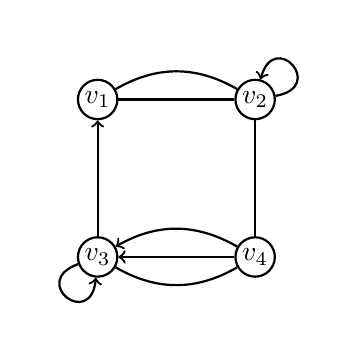
\begin{tikzpicture}
    \tikzset{punkt/.style={circle, thick, draw=black, minimum width=0.5cm,inner sep=0}}
    \node[punkt] at (0,0)      (v1){$v_1$};
    \node[punkt] at (2,0)      (v2){$v_2$};
    \node[punkt] at (0,-2)     (v3){$v_3$};
    \node[punkt] at (2,-2)      (v4){$v_4$};
    
    \draw [-, thick, draw=black] (v1) -- (v2);
    \draw [<-, thick, draw=black] (v1) -- (v3);
    \draw [-, thick, draw=black] (v2) -- (v4);
    \draw [<-, thick, draw=black] (v3) -- (v4);
    \draw [-, thick, draw=black] (v1) to[bend left] (v2);
    \draw [-, thick, draw=black] (v3) to[bend right] (v4);
    \draw [<-, thick, draw=black] (v3) to[bend left] (v4);
    \path  (v2)  edge[->, out=10,in=75,looseness=6, thick, draw=black] (v2);
    \path  (v3)  edge[->, out=200,in=265,looseness=6, thick, draw=black] (v3);
  \end{tikzpicture}
  \captionof{figure}{En blandet graf.}
  \label{fig:Graf123}
\end{center}

%Et polyhedron er derfor en samling af polyeder der til sammen skaber en geometrisk figur i et givet vektorrum.
%ligeldes bør der nævnes noget med at a står vinkelret på linjen 